\section{Reference management}

\begin{frame}
  Reference management.
\end{frame}

\subsection{Reference management software}

\begin{frame}
  \frametitle{Reference management}
    \begin{columns}
      \begin{column}{0.5\textwidth}
        What do researches do with bibliographic
        references?~\cite{rongilmour2011}
        \begin{itemize}
          \item Import them from databases.
          \item Organize them.
          \item Gather additional metadata.
          \item Highlight and add notes to them.
          \item Sharing them.
          \item Convert them between formats or styles.
          \item Insert them to documents using word processing software.
        \end{itemize}
      \end{column}
      \begin{column}{0.5\textwidth}
        \begin{figure}
          \centering
          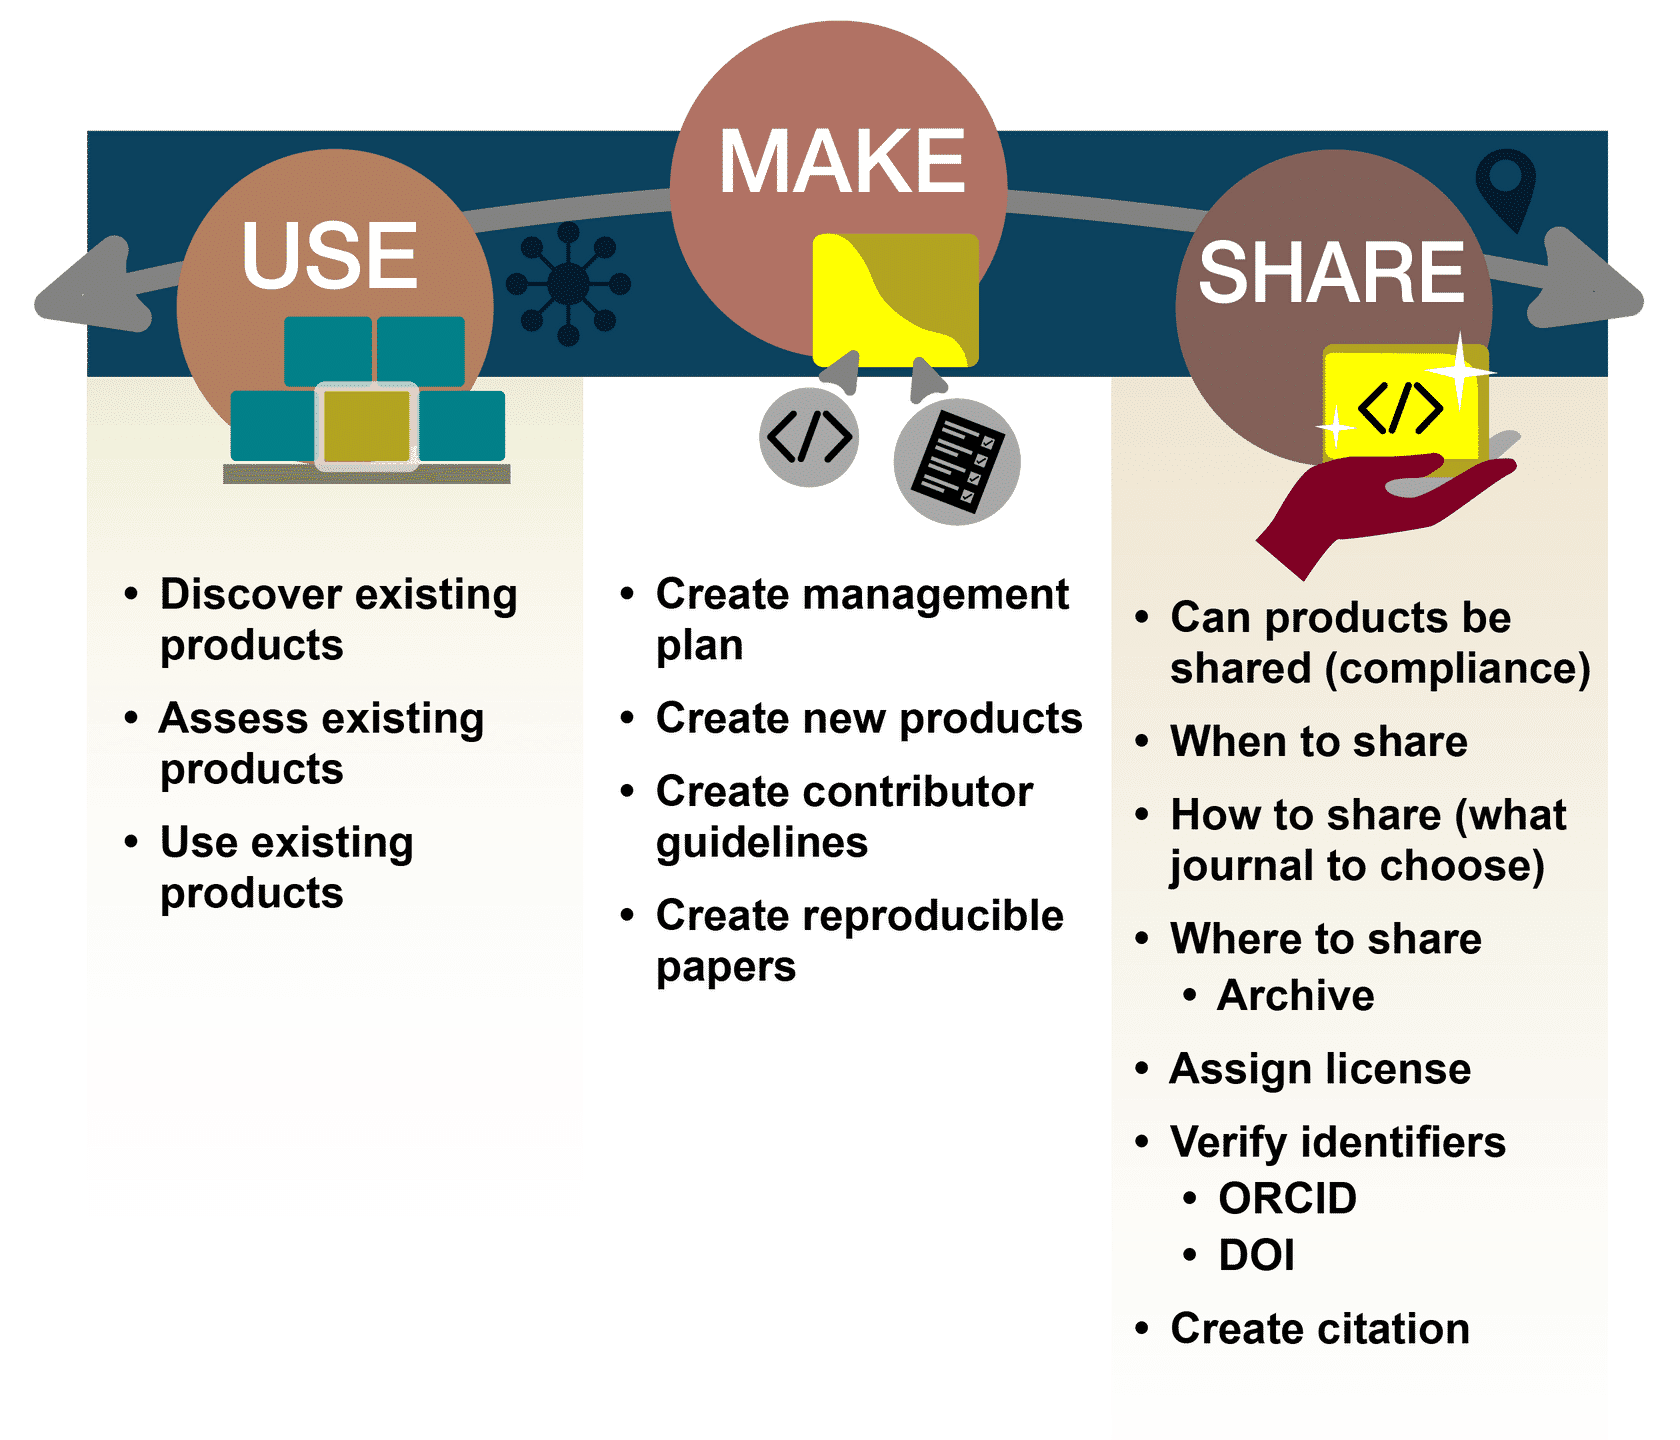
\includegraphics[width=0.97\textwidth]{images/use_make_share.png}
          \label{fig:use_make_share}
          \caption{
            Source:
            \href{https://stemgateway.nasa.gov/s/course-offering/a0BSJ0000049ih3/open-science-101}{OpenScience101.org}
            ~\cite{nasatopsopenscience101}.
          }
        \end{figure}
      \end{column}
    \end{columns}
\end{frame}

\begin{frame}[label={tools-reference-management}]
  \frametitle{Tools for reference management}  
      \begin{columns}
        \begin{column}{0.5\textwidth}
      \begin{itemize}
        \item There are at least 15 pieces of software for reference management.
        \item \citeauthor{rongilmour2011} made a comparison between
          CiteULike, RefWorks, Mendeley, and Zotero~\cite{rongilmour2011} in
          2011.
        \item For a more up-to-date comparison, also check
          \href{https://en.wikipedia.org/wiki/Comparison_of_reference_management_software}
          {software comparison article in Wikipedia.}
      \end{itemize}
    \end{column}
    \begin{column}{0.5\textwidth}
      \begin{figure}
        \centering
        
\includegraphics[scale=0.3]{images/RTFM_coffee_mug.jpg}
        \caption{Google is your friend. Source:~
          \href{https://en.wikipedia.org/w/index.php?title=Google_is_your_friend&redirect=no}
          {Wikipedia}}
      \end{figure}
    \end{column}
  \end{columns}
\end{frame}

\subsection{Zotero}

\begin{frame}
  \frametitle{Zotero}
  \begin{columns}
    \begin{column}{0.5\textwidth}
      \begin{itemize}
        \item Free and open source reference management software
        (AGPL v3 license).
        \item Free cloud storage up to 300 MB. 
        \item Released in 2006.
        \item Commonly used in medicine~\cite{mueenahmed2011,vanhecke2008}.
        \item Integration with Word Processor Software (MS Word, LibreOffice
          Writer, OnlyOffice, and Google docs).
        \item Integration with Web Browsers (Firefox, Chrome, Safari, Edge).
      \item Download \href{https://www.zotero.org/download/}{here}.
      \end{itemize}
    \end{column}
    \begin{column}{0.5\textwidth}
      \begin{figure}
        \centering
        
\includegraphics[scale=0.7]{logos/logo_zotero.png}
      \end{figure}
    \end{column}
  \end{columns}
\end{frame}

\begin{frame}
  \frametitle{Import references to Zotero}
  \begin{columns}
    \begin{column}{0.5\textwidth}
      Import references from other software:
      \begin{itemize}
        \item Mendeley.
        \item EndNote.
        \item Citavi.
        \item MS Word bibliography XML.
        \item Plain text.
        \item Bib(La)Tex.
        \item JabRef.
        \item Check how
          \href{https://www.zotero.org/support/moving_to_zotero}{here}.
      \end{itemize}
    \end{column}
    \begin{column}{0.5\textwidth}
      \begin{figure}
        \centering
        
\includegraphics[scale=0.4]{logos/citavi-all-logo-300x106.png}
        
\includegraphics[scale=0.25]{logos/EndNote.png}
        
\includegraphics[scale=0.3]{logos/Mendeley.png}
        
\includegraphics[scale=0.02]{logos/Microsoft-Word-Symbol.png}
      \end{figure}
    \end{column}
  \end{columns}
\end{frame}

\begin{frame}
  \frametitle{Organize references into collections}
  \begin{columns}
    \begin{column}{0.5\textwidth}
      \begin{itemize}
        \item References can be organized into collections.
        \item Collections allow hierarchical organization.
        \item The same item (reference) can belong to multiple collections.
        \item Use drag and drop to add items to collections.
        \item The TREESLab library has a collection for each project.
      \end{itemize}
    \end{column}
    \begin{column}{0.5\textwidth}
      \begin{figure}
        \centering
        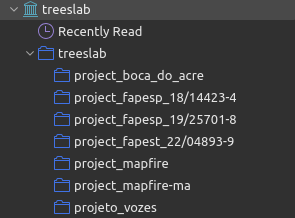
\includegraphics[scale=0.6]{images/treeslab_zotero_collections.png}
      \end{figure}
    \end{column}
  \end{columns}
\end{frame}

\begin{frame}
  \frametitle{Gather additional metadata}
  \begin{columns}
    \begin{column}{0.5\textwidth}
      \begin{itemize}
        \item Zotero allows you to fill additional metadata for each item.
        \item You can even associate a PDF to an item (reference) in Zotero.
      \end{itemize}
    \end{column}
    \begin{column}{0.5\textwidth}
      \begin{figure}
        \centering
        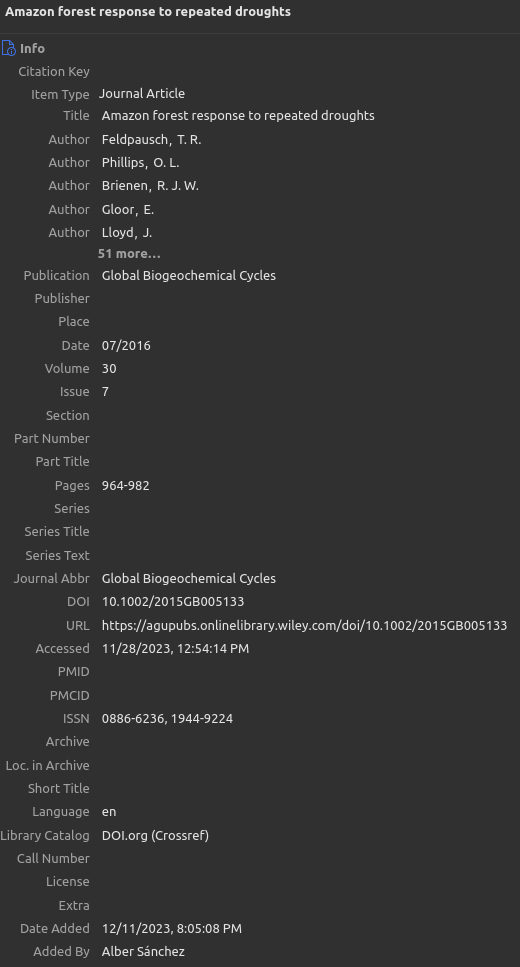
\includegraphics[scale=0.20]{images/treeslab_example.png}
      \end{figure}
    \end{column}
  \end{columns}
\end{frame}

\begin{frame}
  \frametitle{Highlight and add notes to references}
  \begin{columns}
    \begin{column}{0.5\textwidth}
      \begin{itemize}
        \item Zotero allows you to highlight and add notes to a PDF associated
          to an item (reference).
        \item You can also add notes to your highlights, to a (help \href{https://www.zotero.org/support/notes}{here}).
      \end{itemize}
    \end{column}
    \begin{column}{0.5\textwidth}
      \begin{figure}
        \centering
        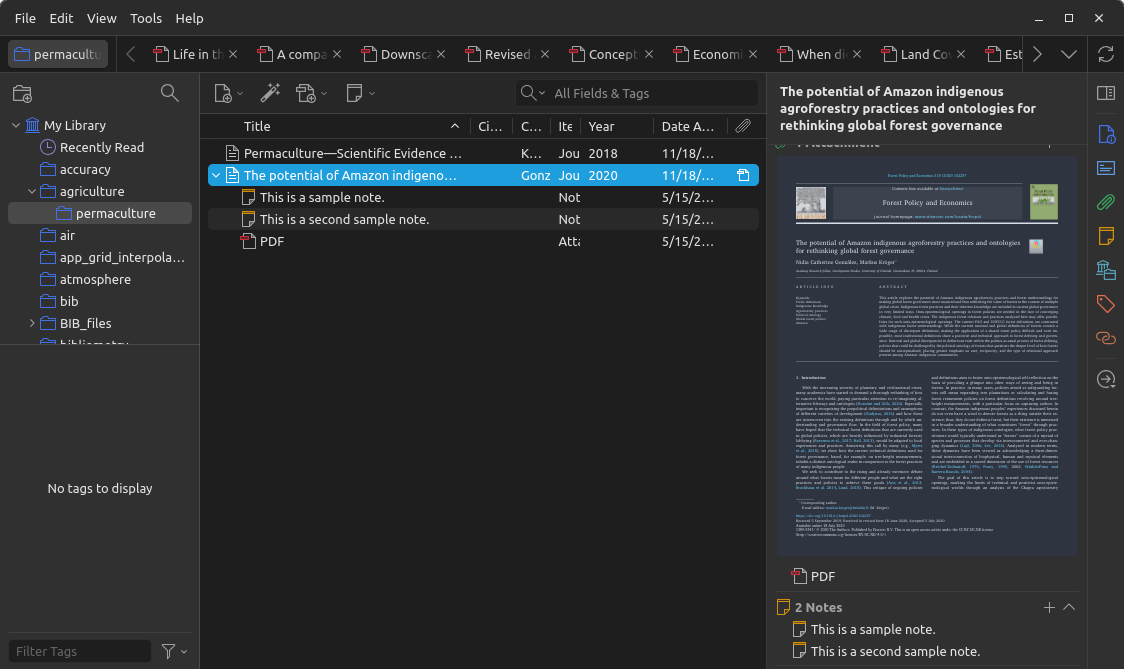
\includegraphics[scale=0.19]{images/zotero_pdf_notes.png}
      \end{figure}
    \end{column}
  \end{columns}
\end{frame}

\begin{frame}
  \frametitle{Share references}
  \begin{columns}
    \begin{column}{0.5\textwidth}
      \begin{itemize}
        \item Zotero allows you to create groups and use them to share references
          with colleagues.
        \item The TREESLab' publication list is a collection associated with the
          Zotero group called \textit{treeslab}.
      \end{itemize}
    \end{column}
    \begin{column}{0.5\textwidth}
      \begin{figure}
        \centering
        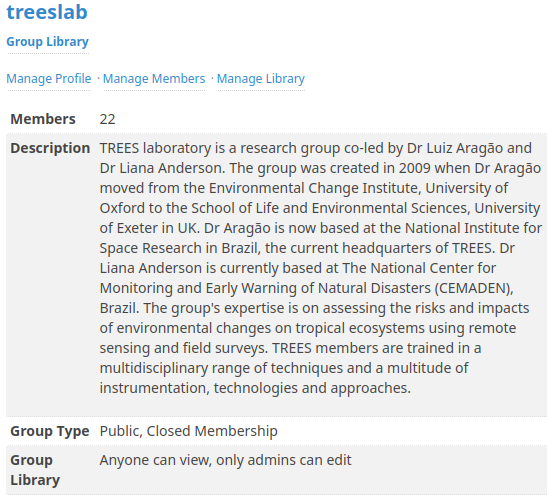
\includegraphics[scale=0.35]{images/treeslab_zotero_group.png}
      \end{figure}
    \end{column}
  \end{columns}
\end{frame}

\begin{frame}[label={convert_styles}]
  \frametitle{Convert references between formats or styles}
  \begin{columns}
    \begin{column}{0.5\textwidth}
      \begin{itemize}
        \item Zotero allows you to export items (references) or collections
          to several formats.
        \item It also allows to copy references and format them according
          to several reference styles.
        \item It is possible to add the ABTN style from
          \href{https://www.zotero.org/styles?q=abnt}{here}.
      \end{itemize}
    \end{column}
    \begin{column}{0.5\textwidth}
      \begin{figure}
        \centering
        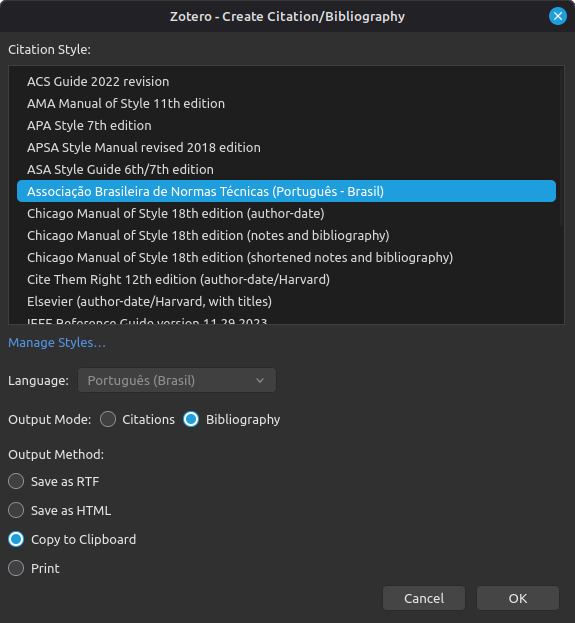
\includegraphics[scale=0.25]{images/zotero_citation_styles.png}
      \end{figure}
    \end{column}
  \end{columns}
\end{frame}

\begin{frame}
  \frametitle{Insert references into text documents}
  \begin{columns}
    \begin{column}{0.5\textwidth}
      \begin{itemize}
        \item \href{https://www.zotero.org/support/google_docs}{Google Docs} (using
          the Zotero connector for Web Browsers).
        \item \href{https://www.zotero.org/support/libreoffice_writer_plugin_usage}
          {Libre Office}.
        \item LaTeX (export collection to a BIB file).
        \item \href{https://www.zotero.org/support/word_processor_plugin_usage}
          {MS Word}.
      \end{itemize}
    \end{column}
    \begin{column}{0.5\textwidth}
      \begin{figure}
        
\includegraphics[scale=0.5]{logos/libreoffice-tdf-logo.png} \\
        \vspace{0.9cm}
        
\includegraphics[scale=0.3]{logos/Latex-Logo-Vector.png}
      \end{figure}
    \end{column}
  \end{columns}
\end{frame}

\begin{frame}[label=google_docs_zotero]
  \frametitle{Google Docs and Zotero}
  \begin{columns}
    \begin{column}{0.5\textwidth}
      \begin{itemize}
        \item Download the connector from
          \href{https://www.zotero.org/download/}{here}.
        \item Grant Google access to your Zotero account.
        \item Choose a style for your references.
        \item The Zotero menu in the tool bar is activated.
        \item Make sure your Zotero desktop instance is running.
        \item Add references to your text.
        \item Add a bibliography section.
      \end{itemize}
    \end{column}
    \begin{column}{0.5\textwidth}
      \begin{figure}
        \centering
        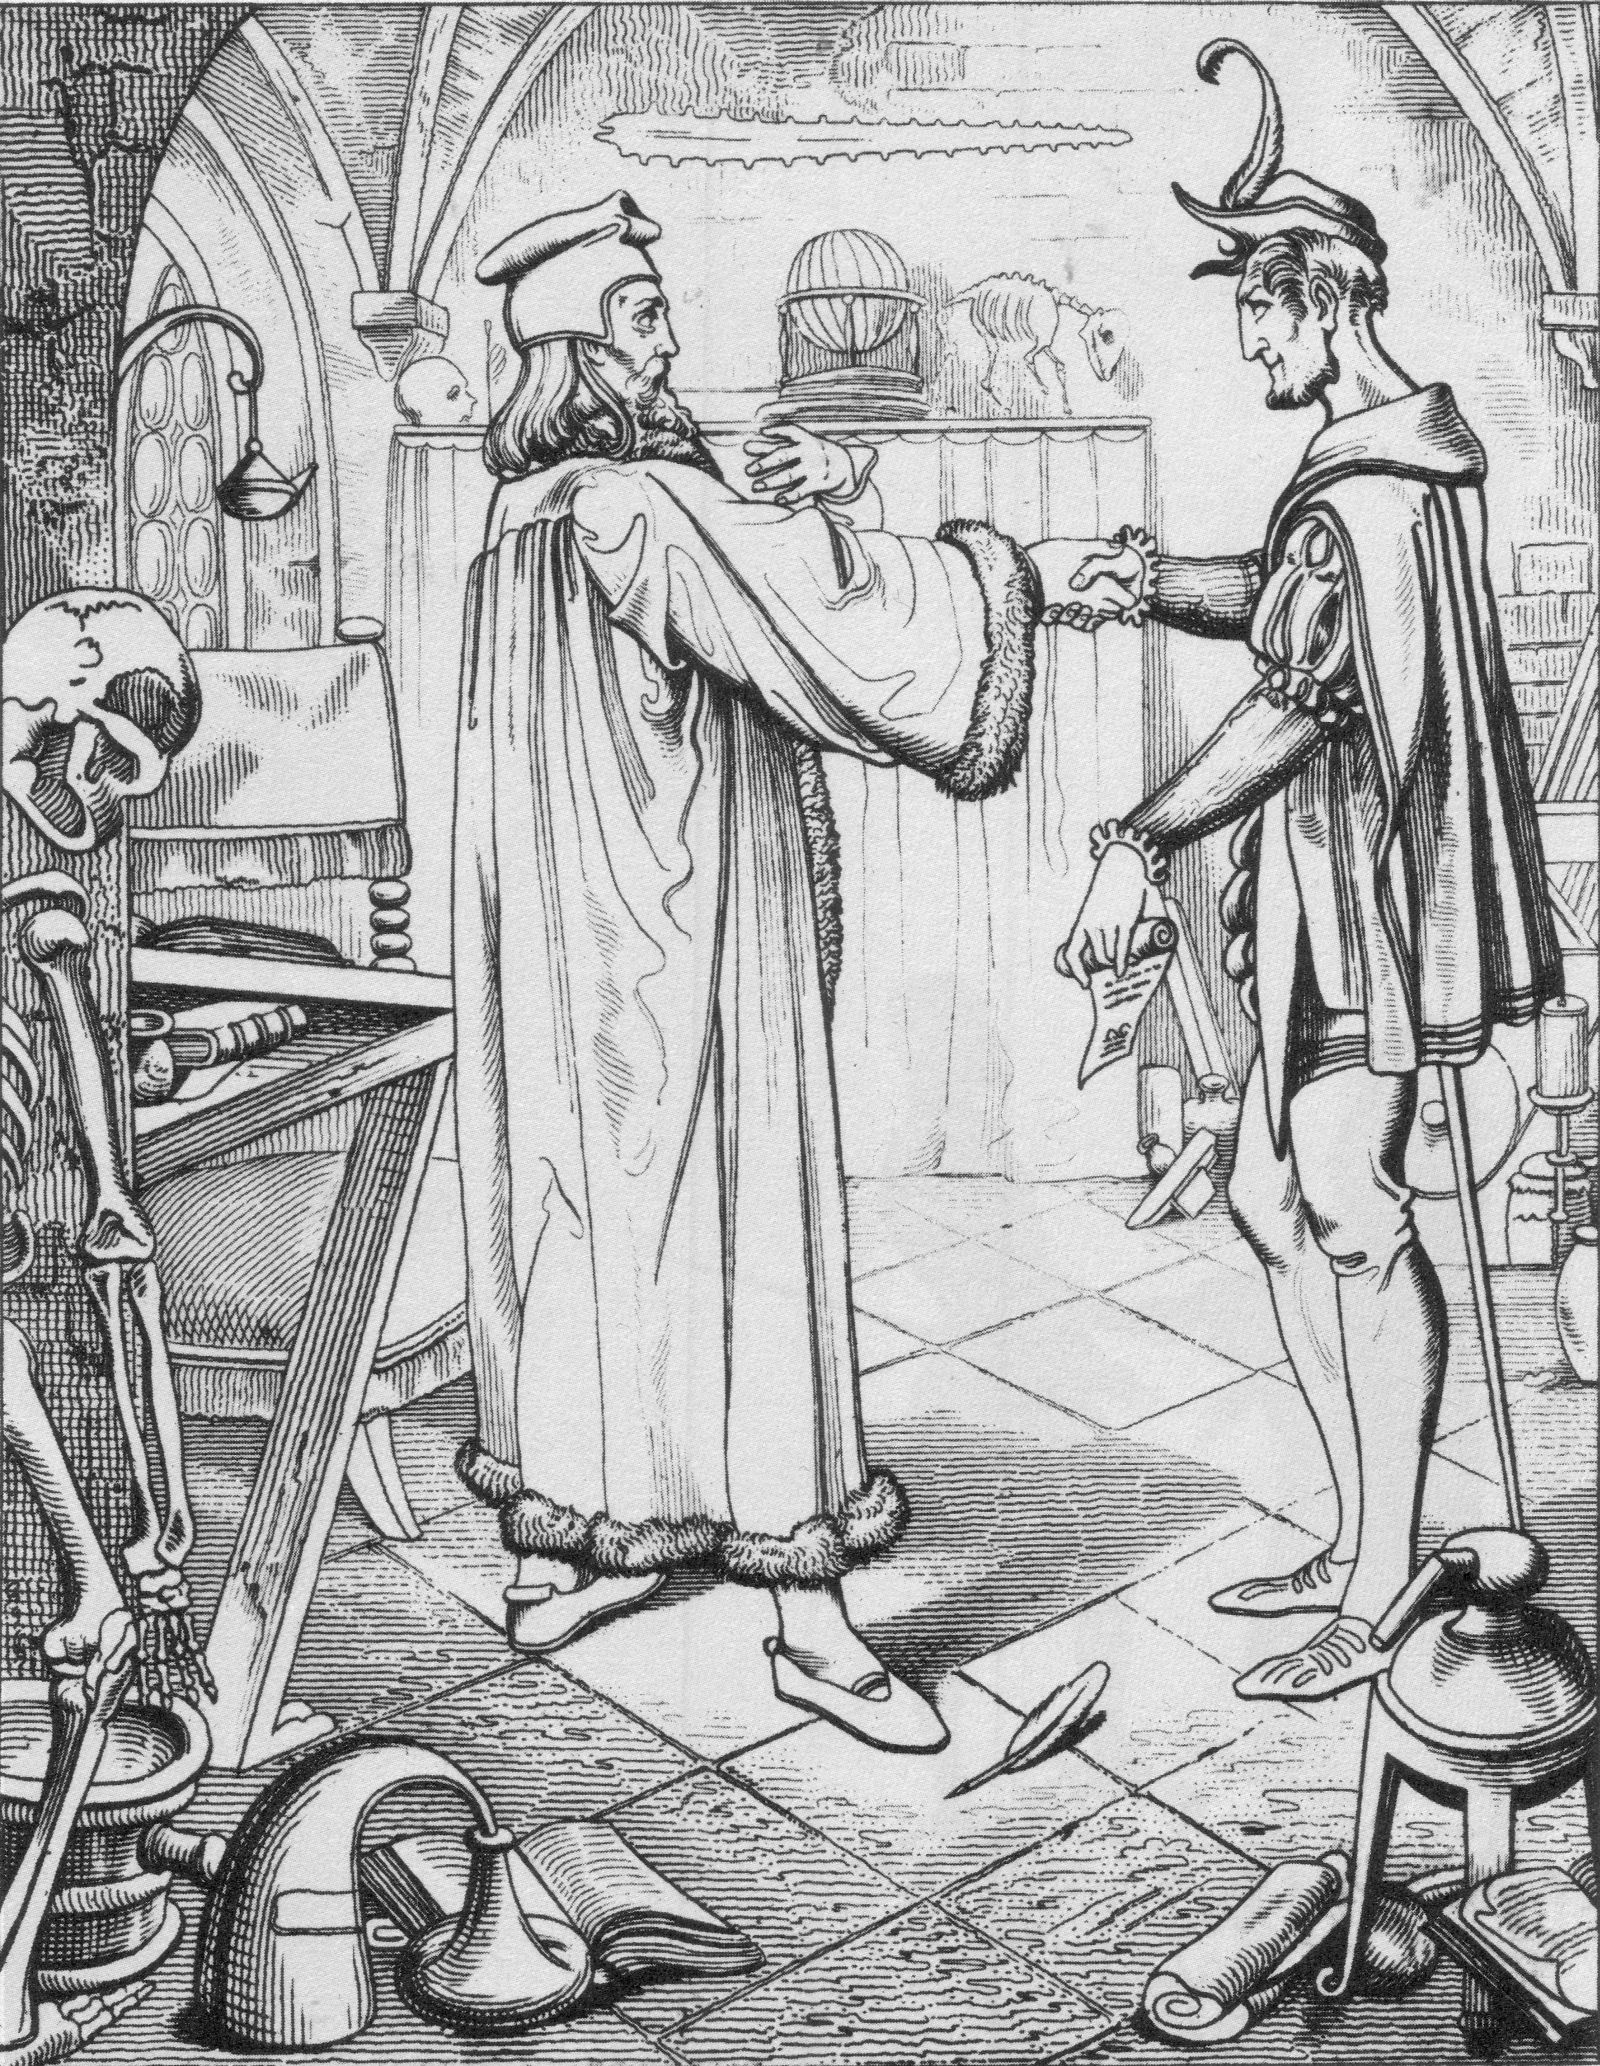
\includegraphics[scale=0.7]
        {images/Teufelspakt_Faust-Mephisto,_Julius_Nisle.jpg}
        \caption{Faustian bargain.
        Source:~\href{https://en.wikipedia.org/wiki/Deal_with_the_Devil}
        {Wikipedia}}
      \end{figure}
    \end{column}
  \end{columns}
\end{frame}

\subsection{Zotero and TREESLab}

\begin{frame}
  \frametitle{TREESLab group at Zotero}
  \begin{columns}
    \begin{column}{0.5\textwidth}
      \begin{itemize}
        \item TREESLab has a Zotero group (click
          \href{https://www.zotero.org/groups/5304570/treeslab}{here}).
        \item This group hosts TREESLab's publication list.
        \item The group owner is TREESLab's email account
          \href{mailto:wertreeslab@gmail.com}{wertreeslab@gmail.com}
        \item Here we keep track of the publications produced by TREESLab.
        \item TREESLab members don't have to be members to add their
          publications to the list (but it'd be nice, though).
      \end{itemize}
    \end{column}
    \begin{column}{0.5\textwidth}
      \begin{figure}
        \centering
        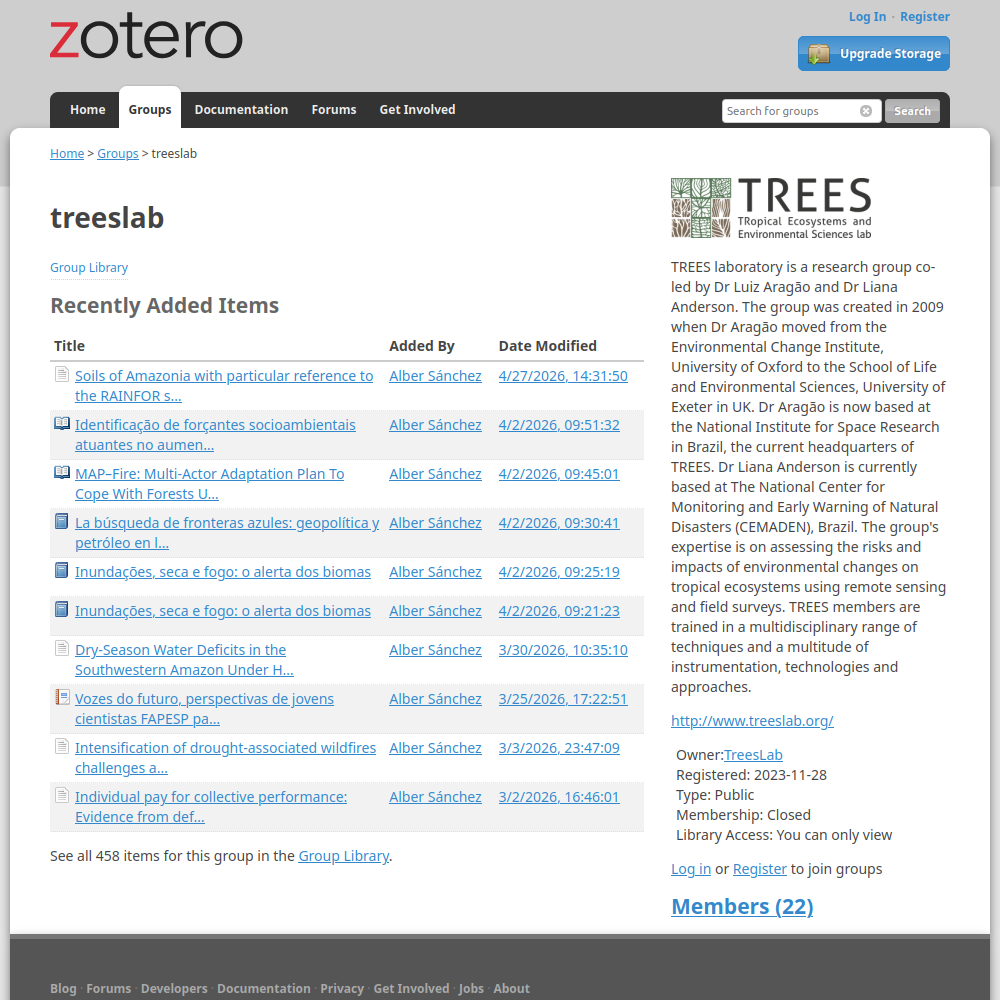
\includegraphics[scale=0.20]{images/zotero_group_treeslab.png}
      \end{figure}
    \end{column}
  \end{columns}
\end{frame}

\begin{frame}
  \frametitle{Researcher's profile at \url{zotero.org}}
  \begin{columns}
    \begin{column}{0.5\textwidth}
      \begin{itemize}
        \item Researchers can build a profile and \url{zotero.org} will host it.
        \item This profile would display the items in the
          \textit{My Publicatons} collection (check \href{https://www.zotero.org/support/my_publications}{here}).
      \end{itemize}
    \end{column}
    \begin{column}{0.5\textwidth}
      \begin{figure}
        \centering
        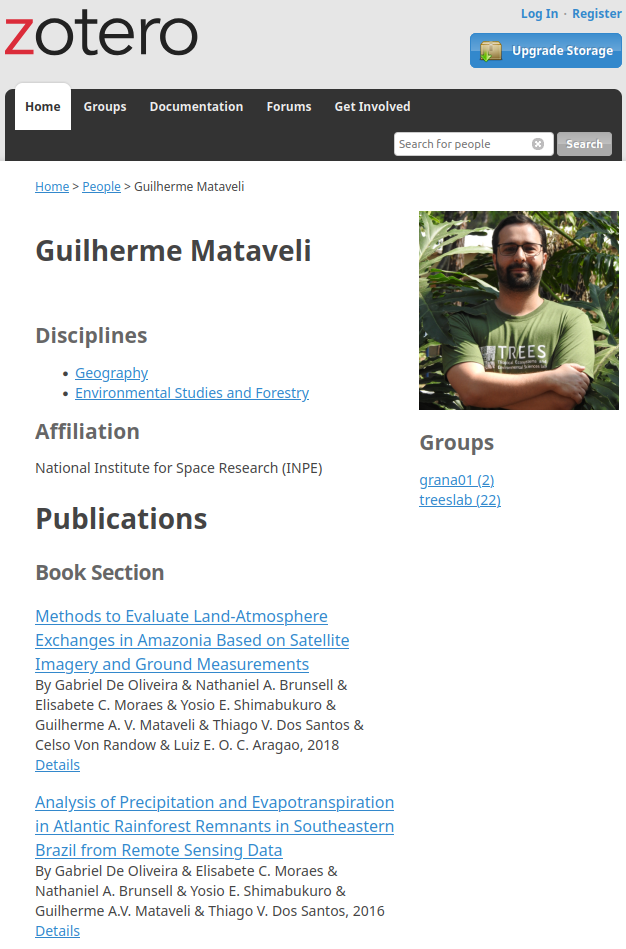
\includegraphics[scale=0.19]{images/zotero_guilherme_mataveli.png}
        \caption{A researcher's profile. Source:
        \href{https://www.zotero.org/gmataveli}{zotero.org}.}
      \end{figure}
    \end{column}
  \end{columns}
\end{frame}

\begin{frame}
  \begin{figure}
    \centering
    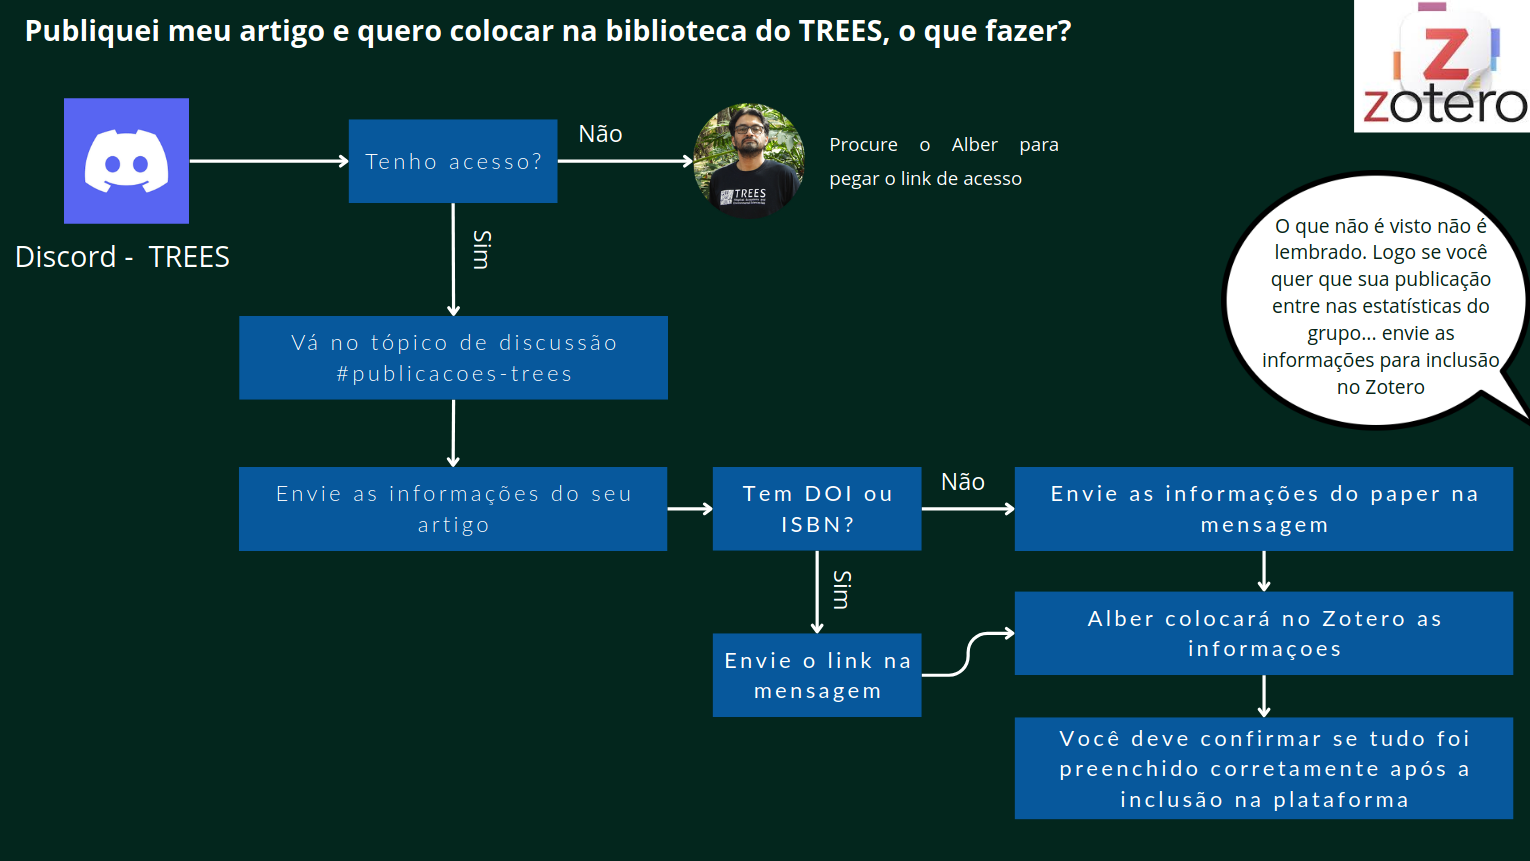
\includegraphics[scale=0.275]{images/zotero_treeslab_add.png}
  \end{figure}
\end{frame}

\begin{frame}
  \frametitle{Questions}
  \begin{itemize}
    \item \textit{Dificuldade de personalizar referências}
      \begin{itemize}
        \item Check slide~\ref{convert_styles}. \end{itemize}
    \item \textit{Como vincular ao Google Docs }
      \begin{itemize}
        \item Check slide~\ref{google_docs_zotero}.
      \end{itemize}
    \item \textit{Qual a vantagem do Zotero em relação ao Mendeley?}
      \begin{itemize}
        \item Check slide~\ref{tools-reference-management}.
      \end{itemize}
  \end{itemize}
\end{frame}
